\chapter{Vibrazioni reticolari}

Fino a questo punto abbiamo discusso il comportamento degli elettroni in un cristallo assumendo i nuclei fissi nelle loro posizioni reticolari. In realtà i nuclei non sono mai veramente fermi: compiono \textbf{vibrazioni} attorno alle proprie posizioni di equilibrio, indotte dall'agitazione termica o dalla propagazione di energia nel materiale, che si traducono in una modifica continua della loro posizione.

Il fenomeno costituisce al tempo stesso un \emph{problema} e un \emph{vantaggio}:

\begin{itemize}
    \item l'oscillazione dei nuclei attorno alla posizione di equilibrio dipende dalla temperatura \( T \) e può limitare la conduzione di corrente, perché i portatori subiscono uno scattering aggiuntivo dovuto al reticolo non più statico;
    \item d'altra parte, le vibrazioni reticolari sono responsabili della propagazione delle onde meccaniche e sonore nel materiale, e ne determinano molte proprietà termiche.
\end{itemize}

Per analizzare il problema sfruttiamo in modo essenziale la struttura periodica del cristallo. Consideriamo una famiglia di piani cristallini paralleli, indicati con \( \pi \), separati da una distanza interplanare \( a \).

\begin{figure}[htbp]
    \centering
    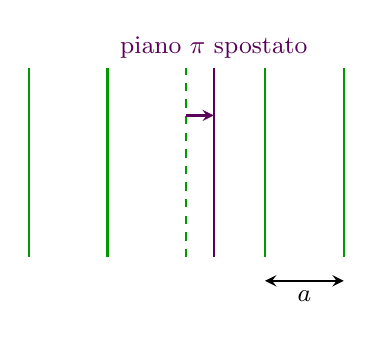
\begin{tikzpicture}[>=stealth, scale=1.0]
        % Equilibrium planes (vertical lines)
        \foreach \x in {-2, -1, 1, 2} {
            \draw[thick, green!60!black] (\x, -1.2) -- (\x, 1.2);
        }
        % Displaced plane (shifted to the right of equilibrium at x=0)
        \draw[thick, green!60!black, dashed] (0, -1.2) -- (0, 1.2);
        \draw[thick, violet!70!black] (0.35, -1.2) -- (0.35, 1.2);
        \draw[->, violet!70!black, thick] (0, 0.6) -- (0.35, 0.6);

        % Distance label "a"
        \draw[<->, thick] (1, -1.5) -- (2, -1.5);
        \node[anchor=north, font=\small] at (1.5, -1.5) {\( a \)};

        \node[anchor=south, font=\small, violet!70!black] at (0.35, 1.2) {piano \( \pi \) spostato};
    \end{tikzpicture}
    \caption{Famiglia di piani cristallini paralleli, separati dalla distanza interplanare \( a \). Uno dei piani è rappresentato spostato dalla sua posizione di equilibrio.}
    \label{fig:piani_cristallini_vibrazioni}
\end{figure}

Se uno dei piani viene perturbato e si sposta dalla sua posizione di equilibrio, la sua oscillazione si \emph{riflette} sui piani adiacenti, che a loro volta vengono messi in moto. Supponiamo che la perturbazione sia sufficientemente piccola da non modificare in modo permanente la struttura del materiale, in modo che il cristallo non si rompa e i piani si limitino a oscillare attorno alla loro posizione originale. La vibrazione del piano \( \pi \) si propaga allora ai piani adiacenti della stessa famiglia.

Per descrivere il moto introduciamo, per ciascun piano della famiglia, una variabile scalare \( u_s \) che rappresenta la \emph{proiezione} lungo l'asse perpendicolare ai piani dello spostamento del piano stesso dalla posizione di equilibrio. Indichiamo con \( sa \) la posizione di equilibrio dell'\( s \)-esimo piano, in modo che i piani adiacenti si trovino in \( (s-1)a \) e \( (s+1)a \).

\begin{figure}[htbp]
    \centering
    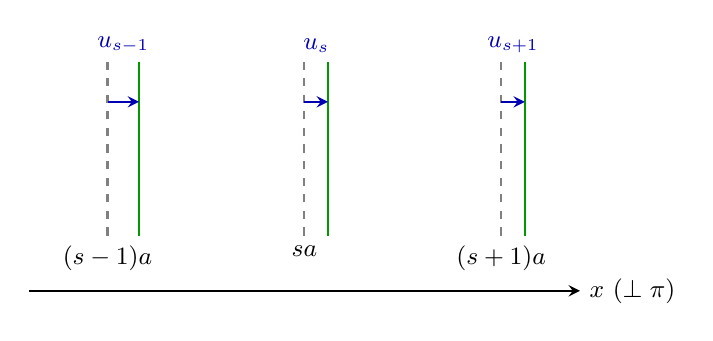
\begin{tikzpicture}[>=stealth, scale=1.0]
        % Equilibrium positions (vertical dashed lines)
        \foreach \x/\lbl in {-2.5/{(s-1)a}, 0/{sa}, 2.5/{(s+1)a}} {
            \draw[thick, dashed, gray] (\x, -1) -- (\x, 1.2);
            \node[anchor=north, font=\small] at (\x, -1) {\( \lbl \)};
        }
        % Displaced planes (solid) with arrows
        \draw[thick, green!60!black] (-2.1, -1) -- (-2.1, 1.2);
        \draw[thick, green!60!black] (0.3, -1) -- (0.3, 1.2);
        \draw[thick, green!60!black] (2.8, -1) -- (2.8, 1.2);

        \draw[->, blue!70!black, thick] (-2.5, 0.7) -- (-2.1, 0.7);
        \draw[->, blue!70!black, thick] (0, 0.7) -- (0.3, 0.7);
        \draw[->, blue!70!black, thick] (2.5, 0.7) -- (2.8, 0.7);

        \node[anchor=south, font=\small, blue!70!black] at (-2.3, 1.2) {\( u_{s-1} \)};
        \node[anchor=south, font=\small, blue!70!black] at (0.15, 1.2) {\( u_s \)};
        \node[anchor=south, font=\small, blue!70!black] at (2.65, 1.2) {\( u_{s+1} \)};

        % Axis
        \draw[->, thick] (-3.5, -1.7) -- (3.5, -1.7);
        \node[anchor=west, font=\small] at (3.5, -1.7) {\( x \) (\( \perp \pi \))};
    \end{tikzpicture}
    \caption{Spostamenti \( u_{s-1} \), \( u_s \), \( u_{s+1} \) dei piani adiacenti rispetto alle proprie posizioni di equilibrio \( (s-1)a \), \( sa \), \( (s+1)a \), proiettati lungo l'asse perpendicolare ai piani.}
    \label{fig:spostamenti_piani}
\end{figure}

Sfruttiamo a questo punto le \textbf{proprietà di simmetria} del cristallo: tutti i piani della famiglia \( \{\pi\} \) sono equivalenti dal punto di vista strutturale, e altrettanto lo sono gli atomi che li compongono. Il moto della famiglia di piani \( \{\pi\} \) può quindi essere tradotto nel moto degli atomi appartenenti a \( \{\pi\} \), che possiedono caratteristiche strutturali identiche. In questo modo, da un problema intrinsecamente tridimensionale e a molti corpi, riusciamo a passare a un problema effettivamente \emph{unidimensionale}, descritto dalle sole variabili \( u_s \) lungo la direzione perpendicolare ai piani.

Cerchiamo allora una soluzione di tipo ondulatorio per lo spostamento dell'\( s \)-esimo piano. La forma più naturale è quella di un'onda piana:

\begin{equation}
    X_s(t) = A_0 \, e^{i k s a} \, e^{-i \omega t},
\end{equation}

dove ciascun fattore ha un significato fisico ben preciso:

\begin{itemize}
    \item \( A_0 \) è l'\textbf{ampiezza} dell'oscillazione;
    \item \( e^{i k s a} \) fissa la \emph{posizione di equilibrio} del componente del piano \( \pi \) lungo la direzione \( x \), attraverso il vettore d'onda \( k \) e l'indice intero \( s \);
    \item \( e^{-i \omega t} \) è la \emph{componente oscillante nel tempo}, di pulsazione \( \omega \).
\end{itemize}

L'oscillazione attorno alla posizione di equilibrio è dunque quella di un \textbf{oscillatore armonico}. Analogamente si scrivono gli spostamenti dei piani adiacenti:

\begin{align}
    X_{s-1}(t) &= A_0 \, e^{i k (s-1) a} \, e^{-i \omega t}, \\
    X_{s+1}(t) &= A_0 \, e^{i k (s+1) a} \, e^{-i \omega t}.
\end{align}

Riassumendo, il problema tridimensionale dei nuclei in un cristallo si è ridotto a quello di una \textbf{catena lineare} di atomi: ciascun piano è rappresentato da un singolo punto sulla retta, posto nella propria posizione di equilibrio \( (s-1)a, \, sa, \, (s+1)a, \, (s+2)a, \, \ldots \), e i piani adiacenti sono accoppiati fra loro tramite un'interazione di tipo elastico.

\begin{figure}[htbp]
    \centering
    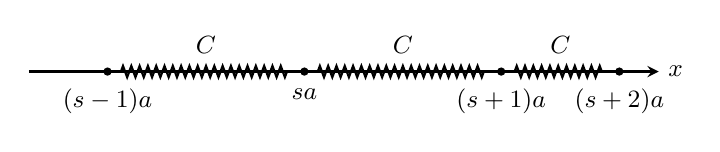
\begin{tikzpicture}[>=stealth, scale=1.0,
        spring/.style={decorate, decoration={zigzag, segment length=3pt, amplitude=2pt, pre length=2pt, post length=2pt}, thick}]
        % Axis
        \draw[->, thick] (-3.5, 0) -- (4.5, 0);
        \node[anchor=west, font=\small] at (4.5, 0) {\( x \)};

        % Equilibrium positions
        \foreach \x/\lbl in {-2.5/{(s-1)a}, 0/{sa}, 2.5/{(s+1)a}, 4/{(s+2)a}} {
            \fill (\x, 0) circle (1.5pt);
            \node[anchor=north, font=\small] at (\x, -0.1) {\( \lbl \)};
        }

        % Springs between atoms
        \draw[spring] (-2.4, 0) -- (-0.1, 0);
        \draw[spring] (0.1, 0) -- (2.4, 0);
        \draw[spring] (2.6, 0) -- (3.9, 0);

        % Spring constant labels
        \node[anchor=south, font=\small] at (-1.25, 0.1) {\( C \)};
        \node[anchor=south, font=\small] at (1.25, 0.1) {\( C \)};
        \node[anchor=south, font=\small] at (3.25, 0.1) {\( C \)};
    \end{tikzpicture}
    \caption{Catena lineare di atomi: ogni piano è ridotto a un punto nella propria posizione di equilibrio, e piani adiacenti sono connessi da una molla di costante elastica \( C \).}
    \label{fig:catena_lineare}
\end{figure}

Tutto l'intorno del singolo piano oscilla e tende a tornare alla configurazione di equilibrio, mettendo a sua volta in oscillazione i piani vicini: il sistema si comporta come se gli atomi fossero collegati da \emph{molle}. Queste molle non sono altro che il modo effettivo di descrivere l'impatto dei \textbf{legami chimici} sullo spostamento dalla posizione di equilibrio: la rigidità del legame, racchiusa nella costante elastica \( C \), determina la forza di richiamo che agisce su ciascun piano quando viene perturbato.

\lezione{23}{19/05/2026}

Possiamo ora scrivere l'equazione del moto per l'\( s \)-esimo piano. Indicando con \( M \) la massa associata al piano e considerando la sola componente lungo \( x \), la forza che agisce sull'\( s \)-esimo piano è dovuta ai due piani adiacenti, ciascuno collegato tramite una molla di costante \( C \):

\begin{equation}
    M \dv[2]{X_s}{t} = C (X_{s+1} - X_s) - C (X_s - X_{s-1}).
\end{equation}

Sostituendo l'ansatz ondulatorio \( X_s(t) = A_0 \, e^{i k_x s a} \, e^{-i \omega t} \) e raccogliendo il fattore comune \( e^{i k_x s a} \, e^{-i \omega t} \) otteniamo

\begin{equation}
    -M \omega^{2} = C \left[ e^{i k_x a} + e^{-i k_x a} - 2 \right].
\end{equation}

Usando l'identità \( e^{i k_x a} + e^{-i k_x a} = 2 \cos(k_x a) \) e la formula di bisezione \( 1 - \cos\theta = 2 \sin^{2}(\theta/2) \), l'equazione si riscrive come

\begin{equation}
    \omega^{2} = -\frac{2C}{M} \left[ \cos(k_x a) - 1 \right],
\end{equation}

ovvero, in forma compatta,

\begin{importantbox}
    \begin{equation}
        \omega^{2} = \frac{4C}{M} \sin^{2}\!\left( \frac{k_x a}{2} \right)
        \quad \Longrightarrow \quad
        \omega = \sqrt{\frac{4C}{M}} \, \abs{\sin\!\left( \frac{k_x a}{2} \right)}.
    \end{equation}
\end{importantbox}

Questa è la \textbf{legge di dispersione} \( \omega = \omega(k) \) per le vibrazioni della catena lineare monoatomica. Il suo significato fisico è il seguente: se sul cristallo si applica una perturbazione esterna con lunghezza d'onda \( \lambda \), e quindi con vettore d'onda di modulo

\begin{equation}
    \abs{k} = \frac{2\pi}{\lambda},
\end{equation}

il sistema risponde oscillando con la pulsazione \( \omega(k) \) fissata dalla relazione di dispersione.

\begin{figure}[htbp]
    \centering
    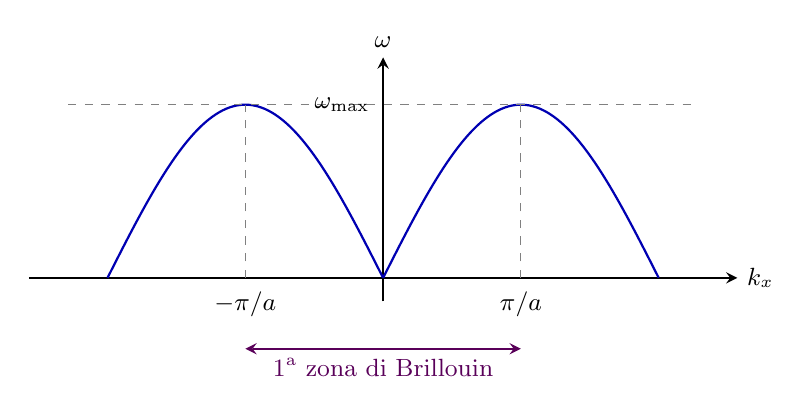
\begin{tikzpicture}[>=stealth, scale=1.0]
        % Axes
        \draw[->, thick] (-4.5, 0) -- (4.5, 0);
        \draw[->, thick] (0, -0.3) -- (0, 2.8);
        \node[anchor=west, font=\small] at (4.5, 0) {\( k_x \)};
        \node[anchor=south, font=\small] at (0, 2.8) {\( \omega \)};

        % First Brillouin zone (central lobe): from -pi/a to pi/a, peak at pi/a... actually peak at pi/a, zero at 0 and 2pi/a
        % |sin(k a /2)| peaks at k = pi/a (sin = 1). Let's plot two lobes: one centered on pi/a (in [0, 2pi/a]) and one on -pi/a
        % Lobe 1: k from -2pi/a to 0, peak at -pi/a
        \draw[thick, blue!70!black, domain=-3.5:0, samples=80, smooth] plot (\x, {2.2*abs(sin(deg(\x*pi/3.5)))});
        % Lobe 2: k from 0 to 2pi/a (use a=3.5/2 scaling)
        \draw[thick, blue!70!black, domain=0:3.5, samples=80, smooth] plot (\x, {2.2*abs(sin(deg(\x*pi/3.5)))});

        % Tick marks at -pi/a, pi/a, -2pi/a hidden
        \draw[dashed, gray] (-1.75, 0) -- (-1.75, 2.2);
        \draw[dashed, gray] (1.75, 0) -- (1.75, 2.2);
        \draw[dashed, gray] (-4, 2.2) -- (4, 2.2);

        \node[anchor=north, font=\small] at (-1.75, -0.05) {\( -\pi/a \)};
        \node[anchor=north, font=\small] at (1.75, -0.05) {\( \pi/a \)};
        \node[anchor=east, font=\small] at (-0.05, 2.2) {\( \omega_{\max} \)};

        % First Brillouin zone bracket
        \draw[<->, violet!70!black, thick] (-1.75, -0.9) -- (1.75, -0.9);
        \node[anchor=north, font=\small, violet!70!black] at (0, -0.9) {1\textsuperscript{a} zona di Brillouin};
    \end{tikzpicture}
    \caption{Relazione di dispersione \( \omega(k_x) \) per la catena lineare monoatomica. Il valore massimo \( \omega_{\max} \) è raggiunto al bordo della prima zona di Brillouin \( k_x = \pm \pi/a \).}
    \label{fig:dispersione_catena_lineare}
\end{figure}

La pulsazione massima si raggiunge al bordo della prima zona di Brillouin, dove \( k_x = \pm \pi/a \):

\begin{equation}
    \omega_{\max} = \sqrt{\frac{4C}{M}} = 2 \sqrt{\frac{C}{M}}.
\end{equation}

La costante elastica \( C \) misura la \emph{forza dei legami chimici} che tengono unito il cristallo: cristalli con legami più rigidi hanno \( C \) più grande, e quindi vibrazioni a frequenze più alte.

La struttura della legge di dispersione riflette in modo manifesto la \textbf{periodicità del cristallo}. Nel reticolo diretto, posizione e vettori primitivi sono

\begin{equation}
    \vec{R} = n \, \vec{a}_1, \qquad \vec{a}_1 = a \, \hat{x}, \qquad n \in \mathbb{Z},
\end{equation}

mentre nel reticolo reciproco

\begin{equation}
    \vec{G} = h \, \vec{b}_1, \qquad \vec{b}_1 = \frac{2\pi}{a} \, \hat{x}, \qquad h \in \mathbb{Z}.
\end{equation}

Tutta l'informazione fisica indipendente è perciò contenuta nella prima zona di Brillouin \( k_x \in [-\pi/a, \pi/a] \): vettori d'onda esterni a questo intervallo sono ricondotti a uno equivalente al suo interno tramite una traslazione di \( \vec{G} \). Per descrivere completamente il comportamento vibrazionale del materiale basta quindi guardare alla prima zona di Brillouin.

È utile analizzare i due regimi limite della relazione di dispersione.

\textbf{Limite delle grandi lunghezze d'onda (\( \abs{k} \to 0 \)).} Quando \( \abs{k} \to 0 \) la lunghezza d'onda \( \lambda \) è molto più grande della distanza interatomica \( a \). In questo regime possiamo approssimare \( \sin(k_x a / 2) \simeq k_x a / 2 \), ottenendo

\begin{equation}
    \omega(k) \simeq \sqrt{\frac{4C}{M}} \, \frac{k_x a}{2} = \left( \sqrt{\frac{C}{M}} \, a \right) k_x.
\end{equation}

La relazione di dispersione è lineare e identifica una \textbf{velocità del suono} nel materiale,

\begin{equation}
    v_s = \sqrt{\frac{C}{M}} \, a,
\end{equation}

cioè la velocità con cui le onde si propagano nel cristallo nel limite del continuo. In questo regime gli atomi adiacenti si muovono \emph{in fase} fra loro: il cristallo si comporta come un mezzo elastico continuo e l'onda lo attraversa senza ``vedere'' la struttura discreta.

\textbf{Limite del bordo zona (\( \abs{k} \to \pi/a \)).} Al bordo della prima zona di Brillouin la pulsazione satura al valore massimo \( \omega \simeq \sqrt{4C/M} \), e la \textbf{velocità di gruppo} si annulla:

\begin{equation}
    v_g = \dv{\omega}{k} = 0.
\end{equation}

Fisicamente questo significa che gli atomi adiacenti di massa \( M \) oscillano in \emph{controfase}, in modo tale che il centro di massa del cristallo rimane fermo e l'onda risulta stazionaria: non c'è propagazione netta di energia attraverso il materiale. Va sottolineato che il moto oscillatorio del singolo atomo, isolato, non coincide con quello di un atomo immerso in una struttura periodica: è proprio l'accoppiamento con i vicini, mediato dalla periodicità, a generare comportamenti collettivi come questo.

\textbf{Accoppiamento con la radiazione elettromagnetica.} Nel limite \( \abs{k} \to 0 \) gli atomi della catena si muovono in fase, con una velocità di gruppo non nulla. In questa configurazione i nuclei, di massa \( M \) molto maggiore di quella elettronica, oscillano lentamente rispetto agli elettroni: la nuvola elettronica si riassesta sui nuovi siti nucleari molto più rapidamente di quanto i nuclei impieghino a spostarsi.

\begin{figure}[htbp]
    \centering
    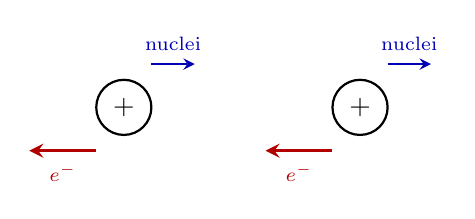
\begin{tikzpicture}[>=stealth, scale=1.0]
        % Two atoms in phase, but electrons move faster
        \draw[thick] (-1.5, 0) circle (0.35);
        \node at (-1.5, 0) {\( + \)};
        \draw[thick] (1.5, 0) circle (0.35);
        \node at (1.5, 0) {\( + \)};

        % Nuclear motion arrows (slow, blue)
        \draw[->, blue!70!black, thick] (-1.15, 0.55) -- (-0.6, 0.55);
        \draw[->, blue!70!black, thick] (1.85, 0.55) -- (2.4, 0.55);
        \node[anchor=south, font=\scriptsize, blue!70!black] at (-0.875, 0.6) {nuclei};
        \node[anchor=south, font=\scriptsize, blue!70!black] at (2.125, 0.6) {nuclei};

        % Electron motion arrows (faster, red, longer)
        \draw[->, red!70!black, very thick] (-1.85, -0.55) -- (-2.7, -0.55);
        \draw[->, red!70!black, very thick] (1.15, -0.55) -- (0.3, -0.55);
        \node[anchor=north, font=\scriptsize, red!70!black] at (-2.275, -0.6) {\( e^{-} \)};
        \node[anchor=north, font=\scriptsize, red!70!black] at (0.725, -0.6) {\( e^{-} \)};
    \end{tikzpicture}
    \caption{Spostamento sfasato tra nuclei ed elettroni durante una vibrazione: gli elettroni si muovono più velocemente dei nuclei, producendo localmente una distribuzione di carica non compensata.}
    \label{fig:dipoli_vibrazione}
\end{figure}

Gli elettroni si muovono dunque \emph{più rapidamente} dei nuclei: localmente si manifestano allora delle \emph{non compensazioni} di carica, perché la nuvola elettronica e quella nucleare non rimangono perfettamente sovrapposte. Si creano in questo modo \textbf{momenti di dipolo} oscillanti nel materiale, alla stessa frequenza delle vibrazioni reticolari.

Questi dipoli oscillanti sono il meccanismo che permette alla radiazione elettromagnetica di accoppiarsi con il materiale: un campo elettromagnetico esterno può mettere in oscillazione i dipoli, trasferendo energia al reticolo, e viceversa vibrazioni reticolari di carattere dipolare possono emettere radiazione elettromagnetica. In sintesi: un campo elettromagnetico applicato genera vibrazioni del reticolo, che a loro volta generano nuovo campo elettromagnetico.

\section{Catena biatomica: un modello più ricco}

Il modello della catena monoatomica cattura l'essenza delle vibrazioni reticolari, ma è troppo semplice per descrivere cristalli reali, in cui la cella primitiva contiene tipicamente più atomi e i legami fra di essi possono avere rigidità diverse. Generalizziamo allora il modello considerando una catena lineare con \textbf{due masse diverse} \( m_1 \) e \( m_2 \) per cella, collegate da molle con \emph{costanti elastiche diverse} \( C \) e \( K \), corrispondenti ai due tipi di legame chimico presenti.

\begin{figure}[htbp]
    \centering
    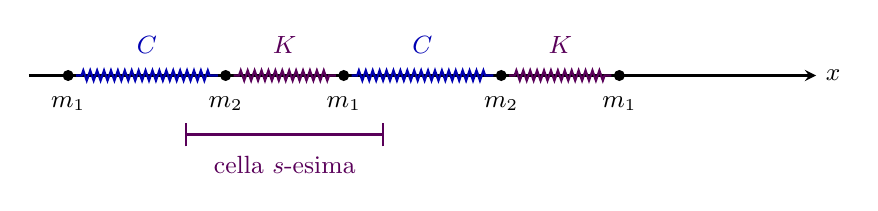
\begin{tikzpicture}[>=stealth, scale=1.0,
        spring/.style={decorate, decoration={zigzag, segment length=2.5pt, amplitude=1.8pt, pre length=2pt, post length=2pt}, thick}]
        % Axis
        \draw[->, thick] (-4.5, 0) -- (5.5, 0);
        \node[anchor=west, font=\small] at (5.5, 0) {\( x \)};

        % Atoms: m_1, m_2, m_1, m_2, m_1
        \foreach \x/\m in {-4/{m_1}, -2/{m_2}, -0.5/{m_1}, 1.5/{m_2}, 3/{m_1}} {
            \fill (\x, 0) circle (2pt);
            \node[anchor=north, font=\small] at (\x, -0.15) {\( \m \)};
        }

        % Springs
        \draw[spring, blue!70!black] (-3.9, 0) -- (-2.1, 0);
        \node[anchor=south, font=\small, blue!70!black] at (-3, 0.15) {\( C \)};

        \draw[spring, violet!70!black] (-1.9, 0) -- (-0.6, 0);
        \node[anchor=south, font=\small, violet!70!black] at (-1.25, 0.15) {\( K \)};

        \draw[spring, blue!70!black] (-0.4, 0) -- (1.4, 0);
        \node[anchor=south, font=\small, blue!70!black] at (0.5, 0.15) {\( C \)};

        \draw[spring, violet!70!black] (1.6, 0) -- (2.9, 0);
        \node[anchor=south, font=\small, violet!70!black] at (2.25, 0.15) {\( K \)};

        % Cell marker for cell s
        \draw[violet!70!black, thick] (-2.5, -0.9) -- (-2.5, -0.6);
        \draw[violet!70!black, thick] (0, -0.9) -- (0, -0.6);
        \draw[violet!70!black, thick] (-2.5, -0.75) -- (0, -0.75);
        \node[anchor=north, font=\small, violet!70!black] at (-1.25, -0.9) {cella \( s \)-esima};
    \end{tikzpicture}
    \caption{Catena biatomica lineare: due masse \( m_1 \) e \( m_2 \) per cella, collegate alternativamente da molle di costante \( C \) e \( K \).}
    \label{fig:catena_biatomica}
\end{figure}

Per ciascuna cella avremo ora \textbf{due moti distinti}, uno per ogni massa. È conveniente indicizzare le posizioni di ogni massa con il numero di cella \( s \), e poi ricondurre tutto a una posizione \emph{assoluta} lungo l'asse \( x \). Nel nostro schema:

\begin{equation}
    \begin{aligned}
        X_{2,s} &= s \, a,         & \qquad X_{1,s} &= (s+1) \, a,    \\
        X_{2,s+1} &= (s+2) \, a,   & \qquad X_{1,s+1} &= (s+3) \, a,
    \end{aligned}
\end{equation}

dove \( a \) è la distanza fra atomi consecutivi (di conseguenza, la cella ha lunghezza \( 2a \)).

Cerchiamo, come prima, soluzioni di tipo ondulatorio: ogni massa oscilla armonicamente con la stessa pulsazione \( \omega \) ma con un'\textbf{ampiezza propria}, \( A_1 \) per la massa \( m_1 \) e \( A_2 \) per la massa \( m_2 \). Otteniamo allora il sistema di equazioni di Newton per le due masse:

\begin{equation}
    \begin{cases}
        \displaystyle m_1 \dv[2]{X_{1,s}}{t} = \sum_i F_{i,x} = -m_1 \omega^{2} X_{1,s}(t), & X_{1,s}(t) = A_1 \, e^{i k_x (s+1) a} \, e^{-i \omega t}, \\[1.2em]
        \displaystyle m_2 \dv[2]{X_{2,s}}{t} = \sum_j F_{j,x} = -m_2 \omega^{2} X_{2,s}(t), & X_{2,s}(t) = A_2 \, e^{i k_x s a} \, e^{-i \omega t}.
    \end{cases}
\end{equation}

Per rendere il calcolo trattabile in modo simbolico ci limitiamo al caso in cui le due molle hanno la \emph{stessa costante elastica} \( C \), ma massa diversa \(m_1 \neq m_2\): il caso più generale con \( K \neq C \) si tratta in modo del tutto analogo, ma appesantisce inutilmente l'algebra senza modificare la struttura qualitativa del risultato. Esplicitando le forze esercitate dai due primi vicini su ciascuna massa, il sistema di Newton diventa:

\begin{equation}
    \begin{cases}
        \displaystyle m_1 \dv[2]{X_{1,s}}{t} = -m_1 \omega^{2} X_{1,s}(t) = C \left[ X_{2,s+1} - X_{1,s} \right] - C \left[ X_{1,s} - X_{2,s} \right], \\[1em]
        \displaystyle m_2 \dv[2]{X_{2,s}}{t} = -m_2 \omega^{2} X_{2,s}(t) = C \left[ X_{1,s} - X_{2,s} \right] - C \left[ X_{2,s} - X_{1,s-1} \right].
    \end{cases}
\end{equation}

Raccogliendo i termini, otteniamo le due equazioni da risolvere:

\begin{equation}
    \begin{cases}
        -m_1 \omega^{2} X_{1,s}(t) = C \left[ X_{2,s+1} + X_{2,s} - 2 X_{1,s} \right], \\[0.6em]
        -m_2 \omega^{2} X_{2,s}(t) = C \left[ X_{1,s} + X_{1,s-1} - 2 X_{2,s} \right].
    \end{cases}
\end{equation}

Sostituiamo ora le soluzioni ondulatorie \( X_{1,s}(t) = A_1 e^{i k_x (s+1) a} e^{-i \omega t} \) e \( X_{2,s}(t) = A_2 e^{i k_x s a} e^{-i \omega t} \) nel sistema. Dividendo ciascuna equazione per la propria esponenziale, le coordinate \( s \) e \( t \) spariscono e ciò che rimane è un sistema algebrico nelle sole ampiezze:

\begin{equation}
    \begin{cases}
        -m_1 \omega^{2} A_1 = C \left[ A_2 \, e^{i k_x a} + A_2 \, e^{-i k_x a} - 2 A_1 \right], \\[0.6em]
        -m_2 \omega^{2} A_2 = C \left[ A_1 \, e^{i k_x a} + A_1 \, e^{-i k_x a} - 2 A_2 \right].
    \end{cases}
\end{equation}

Riconoscendo che \( e^{i k_x a} + e^{-i k_x a} = 2 \cos(k_x a) \), il sistema assume la forma compatta:

\begin{equation}
    \begin{cases}
        -m_1 \omega^{2} A_1 = 2 C A_2 \cos(k_x a) - 2 C A_1, \\[0.6em]
        -m_2 \omega^{2} A_2 = 2 C A_1 \cos(k_x a) - 2 C A_2.
    \end{cases}
\end{equation}

\begin{note}{Una sola pulsazione, due ampiezze}{nota:biatomica_pulsazione_unica}
L'ipotesi cruciale, da non perdere di vista nel seguito, è che le due masse oscillino con la \emph{stessa pulsazione} \( \omega \) e lo \emph{stesso vettore d'onda} \( k_x \), ma con ampiezze \( A_1 \) e \( A_2 \) in generale diverse, da determinare risolvendo insieme le due equazioni del sistema.
\end{note}

Si tratta di un sistema lineare omogeneo nelle incognite \( A_1 \) e \( A_2 \): ammette soluzioni non banali soltanto se si annulla il determinante della matrice dei coefficienti. Imponendo questa condizione si ottiene la \textbf{relazione di dispersione} per la catena biatomica, nella forma biquadratica:

\begin{importantbox}
    \begin{equation}
        m_1 m_2 \, \omega^{4} - 2 C (m_1 + m_2) \, \omega^{2} + 4 C^{2} \left[ 1 - \cos^{2}(k_x a) \right] = 0.
    \end{equation}
\end{importantbox}

Essendo biquadratica in \( \omega \), questa equazione ammette \textbf{due soluzioni distinte} per \( \omega^{2} \), che indichiamo con \( \omega_{+}^{2} \) e \( \omega_{-}^{2} \):

\begin{equation}
    \omega_{+}^{2} = \omega_{+}^{2}(C, m_1, m_2, k_x), \qquad \omega_{-}^{2} = \omega_{-}^{2}(C, m_1, m_2, k_x).
\end{equation}

A ciascun valore del vettore d'onda \( k_x \) corrispondono quindi \emph{due} pulsazioni distinte, che danno luogo a due rami nella relazione di dispersione. Specializziamoci al caso \( m_1 \gg m_2 \) con costante elastica \( C \) uguale per tutti i legami, e tracciamo i due rami nella prima zona di Brillouin: poiché la cella ha lunghezza \( 2a \), la zona si estende ora soltanto da \( -\pi/(2a) \) a \( \pi/(2a) \), ovvero la metà rispetto al caso monoatomico.

\begin{figure}[htbp]
    \centering
    \begin{tikzpicture}[>=stealth, scale=1.6,
        declare function={
            oacu(\x) = sqrt(1.625 * (1 - sqrt(1 - 0.852 * (sin(45*\x))^2)));
            oott(\x) = sqrt(1.625 * (1 + sqrt(1 - 0.852 * (sin(45*\x))^2)));
        }]
        % Axes
        \draw[->, thick] (-2.7, 0) -- (2.9, 0) node[anchor=west, font=\small] {\( k_x \)};
        \draw[->, thick] (0, -0.15) -- (0, 2.4) node[anchor=south, font=\small] {\( \omega \)};

        % BZ boundaries
        \draw[red!70!black, dashed, thick] (-2, 0) -- (-2, 2.05);
        \draw[red!70!black, dashed, thick] (2, 0) -- (2, 2.05);
        \node[anchor=north, font=\small, red!70!black] at (-2, -0.05) {\( -\dfrac{\pi}{2a} \)};
        \node[anchor=north, font=\small, red!70!black] at (2, -0.05) {\( \dfrac{\pi}{2a} \)};
        \node[anchor=north, font=\scriptsize, teal!60!black] at (-1.3, -0.55) {lungh.\ cella \( = 2a \)};

        % Acoustic branch
        \draw[blue!80!black, very thick, smooth, samples=120, domain=-2:2] plot (\x, {oacu(\x)});
        % Optical branch
        \draw[blue!80!black, very thick, smooth, samples=120, domain=-2:2] plot (\x, {oott(\x)});

        % Branch labels (on the curves, inside BZ)
        \node[font=\small, blue!80!black] at (-1.2, 1.08) {\( \omega_{-} \)};
        \node[font=\small, blue!80!black] at (-1.2, 1.95) {\( \omega_{+} \)};

        % Band names (further left, above/below curves)
        \node[font=\scriptsize, teal!60!black, anchor=east] at (-2.1, 1.95) {banda ottica};
        \node[font=\scriptsize, teal!60!black, anchor=east] at (-2.1, 0.75) {banda acustica};

        % Value markers at k=0 (max optical) — push label up and to the right
        \draw[gray!70, dashed, thin] (0, 1.803) -- (1.0, 1.803);
        \node[font=\scriptsize, violet!70!black, anchor=west] at (0.9, 2.2) {\( \max = \sqrt{\dfrac{2C}{m_1} + \dfrac{2C}{m_2}} \)};

        % Value markers at zone boundary
        \draw[gray!70, dashed, thin] (2, 1.5) -- (2.6, 1.5);
        \draw[gray!70, dashed, thin] (2, 1.0) -- (2.6, 1.0);
        \node[font=\scriptsize, violet!70!black, anchor=west] at (2.05, 1.65) {\( \sqrt{\dfrac{2C}{m_2}} \)};
        \node[font=\scriptsize, violet!70!black, anchor=west] at (2.05, 0.85) {val.\ max \( = \sqrt{\dfrac{2C}{m_1}} \)};

        % Gap
        \draw[teal!70!black, very thick, <->] (1.5, 1.0) -- (1.5, 1.5);
        \node[font=\small, teal!70!black, anchor=east] at (1.45, 1.25) {GAP};

        % Linear acoustic region label
        \draw[->, thick, blue!80!black] (0.35, 0.35) -- (0.7, 0.65);
        \node[font=\scriptsize, blue!80!black, anchor=west] at (0.55, 0.3) {\( \omega \approx v k \)};

        % Hypothesis label
        \node[font=\scriptsize, violet!70!black, anchor=west] at (2.3, -0.4) {\( m_1 \gg m_2 \), \( C \) uguale \( \forall \) massa};
    \end{tikzpicture}
    \caption{Relazione di dispersione della catena biatomica nella prima zona di Brillouin.}
    \label{fig:dispersione_biatomica}
\end{figure}

I due rami della dispersione hanno una netta interpretazione fisica. Il ramo \( \omega_{-} \), detto \textbf{ramo acustico}, parte dall'origine con andamento lineare \( \omega \approx v k \): le due masse oscillano \emph{in fase}, come un'unica massa effettiva, e il modo si comporta come un'onda sonora; al bordo zona raggiunge il valore massimo \( \sqrt{2C/m_1} \). Il ramo \( \omega_{+} \), detto \textbf{ramo ottico}, parte invece dal valore massimo \( \sqrt{2C/m_1 + 2C/m_2} \) al centro zona, dove le due masse oscillano in \emph{controfase} lasciando fermo il baricentro della cella, e scende a \( \sqrt{2C/m_2} \) al bordo.

Tra i due rami si apre un intervallo di pulsazioni, fra \( \sqrt{2C/m_1} \) e \( \sqrt{2C/m_2} \), in cui la relazione di dispersione \emph{non ammette soluzioni}: si tratta di una \textbf{regione proibita di pulsazioni}, del tutto analoga al gap energetico che incontreremo per gli elettroni in un cristallo. Se si tenta di indurre nel reticolo una vibrazione con pulsazione \( \omega \) interna a questo gap, l'eccitazione non potrà propagarsi come moto collettivo degli atomi, né in fase né in controfase: nessun modo normale della catena ha quella pulsazione, e l'energia introdotta resta confinata invece di trasformarsi in un'onda viaggiante.

\subsection{Il caso speculare: stesse masse, molle diverse}

Si può ora considerare il limite opposto del modello biatomico: una catena in cui tutte le masse sono \emph{uguali}, ma i legami chimici hanno costanti elastiche \emph{diverse}, alternate lungo la catena. Riprendiamo la geometria della Figura~\ref{fig:catena_biatomica} ponendo \( m_1 = m_2 \equiv m \) e rinominando per chiarezza le due costanti elastiche \( C \) e \( G \), con \( C \neq G \).

\begin{figure}[htbp]
    \centering
    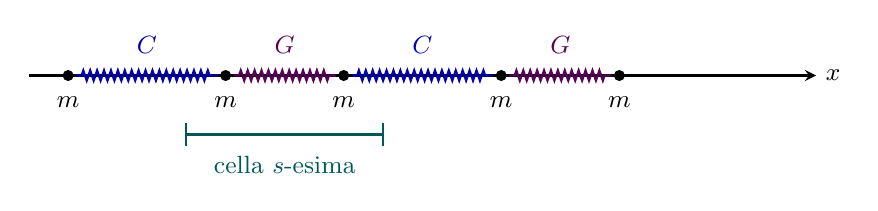
\begin{tikzpicture}[>=stealth, scale=1.0,
        spring/.style={decorate, decoration={zigzag, segment length=2.5pt, amplitude=1.8pt, pre length=2pt, post length=2pt}, thick}]
        \draw[->, thick] (-4.5, 0) -- (5.5, 0);
        \node[anchor=west, font=\small] at (5.5, 0) {\( x \)};

        \foreach \x in {-4, -2, -0.5, 1.5, 3} {
            \fill (\x, 0) circle (2pt);
            \node[anchor=north, font=\small] at (\x, -0.15) {\( m \)};
        }

        \draw[spring, blue!70!black] (-3.9, 0) -- (-2.1, 0);
        \node[anchor=south, font=\small, blue!70!black] at (-3, 0.15) {\( C \)};

        \draw[spring, violet!70!black] (-1.9, 0) -- (-0.6, 0);
        \node[anchor=south, font=\small, violet!70!black] at (-1.25, 0.15) {\( G \)};

        \draw[spring, blue!70!black] (-0.4, 0) -- (1.4, 0);
        \node[anchor=south, font=\small, blue!70!black] at (0.5, 0.15) {\( C \)};

        \draw[spring, violet!70!black] (1.6, 0) -- (2.9, 0);
        \node[anchor=south, font=\small, violet!70!black] at (2.25, 0.15) {\( G \)};

        \draw[teal!70!black, thick] (-2.5, -0.9) -- (-2.5, -0.6);
        \draw[teal!70!black, thick] (0, -0.9) -- (0, -0.6);
        \draw[teal!70!black, thick] (-2.5, -0.75) -- (0, -0.75);
        \node[anchor=north, font=\small, teal!70!black] at (-1.25, -0.9) {cella \( s \)-esima};
    \end{tikzpicture}
    \caption{Catena con masse uguali e costanti elastiche alternate \( C \) e \( G \).}
    \label{fig:catena_masse_uguali}
\end{figure}

La struttura delle equazioni di Newton è identica al caso già trattato:

\begin{equation}
    m \dv[2]{X_{1,s}}{t} = \sum_j F_{j,x},
\end{equation}

con la differenza che ora a cambiare lungo la catena sono le costanti elastiche, non le masse. Ripercorrendo gli stessi passaggi (esplicitazione delle forze, sostituzione delle soluzioni ondulatorie, annullamento del determinante) si ottiene una relazione di dispersione \emph{qualitativamente identica} a quella già discussa: due rami, uno acustico \( \omega_{-} \) ed uno ottico \( \omega_{+} \), separati al bordo della prima zona di Brillouin da un gap di pulsazioni proibite. Al bordo zona i valori limite sono ora, supponendo per esempio \( C > G \):

\begin{equation}
    \omega_{+} \to \sqrt{\frac{2C}{m}}, \qquad \omega_{-} \to \sqrt{\frac{2G}{m}}.
\end{equation}

In altri termini, è la sola presenza di due tipi di legame (o di due tipi di massa) per cella a generare la struttura a due rami con il gap: la cella biatomica è la sorgente fisica del comportamento, indipendentemente da quale dei due parametri (massa o costante elastica) sia quello a variare lungo la catena.

\begin{figure}[htbp]
    \centering
    \begin{tikzpicture}[>=stealth, scale=1.6,
        declare function={
            oacu2(\x) = sqrt(1.625 - sqrt(1.515625 + 1.125 * cos(90*\x)));
            oott2(\x) = sqrt(1.625 + sqrt(1.515625 + 1.125 * cos(90*\x)));
        }]
        % Axes
        \draw[->, thick] (-2.7, 0) -- (2.9, 0) node[anchor=west, font=\small] {\( k_x \)};
        \draw[->, thick] (0, -0.15) -- (0, 2.4) node[anchor=south, font=\small] {\( \omega \)};

        % BZ boundaries
        \draw[red!70!black, dashed, thick] (-2, 0) -- (-2, 2.05);
        \draw[red!70!black, dashed, thick] (2, 0) -- (2, 2.05);

        % BZ marker below axis
        \draw[red!70!black, thick] (-2, -0.5) -- (2, -0.5);
        \draw[red!70!black, thick] (-2, -0.45) -- (-2, -0.55);
        \draw[red!70!black, thick] (2, -0.45) -- (2, -0.55);
        \node[anchor=north, font=\small, red!70!black] at (0, -0.55) {1\textsuperscript{a} zona di Brillouin};

        % Acoustic branch
        \draw[blue!80!black, very thick, smooth, samples=120, domain=-2:2] plot (\x, {oacu2(\x)});
        % Optical branch
        \draw[blue!80!black, very thick, smooth, samples=120, domain=-2:2] plot (\x, {oott2(\x)});

        % Branch labels
        \node[font=\small, blue!80!black] at (-1.2, 1.08) {\( \omega_{-} \)};
        \node[font=\small, blue!80!black] at (-1.2, 1.95) {\( \omega_{+} \)};

        % Band names
        \node[font=\scriptsize, teal!60!black, anchor=east] at (-2.1, 1.95) {banda ottica};
        \node[font=\scriptsize, teal!60!black, anchor=east] at (-2.1, 0.75) {banda acustica};

        % Value markers at zone boundary
        \draw[gray!70, dashed, thin] (2, 1.5) -- (2.6, 1.5);
        \draw[gray!70, dashed, thin] (2, 1.0) -- (2.6, 1.0);
        \node[font=\scriptsize, violet!70!black, anchor=west] at (2.05, 1.65) {\( \sqrt{\dfrac{2C}{m}} \)};
        \node[font=\scriptsize, violet!70!black, anchor=west] at (2.05, 0.85) {\( \sqrt{\dfrac{2G}{m}} \)};

        % Gap
        \draw[teal!70!black, very thick, <->] (1.5, 1.0) -- (1.5, 1.5);
        \node[font=\small, teal!70!black, anchor=east] at (1.45, 1.25) {GAP};
    \end{tikzpicture}
    \caption{Relazione di dispersione della catena con masse uguali e costanti elastiche alternate \( C \neq G \).}
    \label{fig:dispersione_masse_uguali}
\end{figure}

La struttura della Figura~\ref{fig:dispersione_masse_uguali} è la stessa già incontrata nel caso \( m_1 \neq m_2 \): un ramo acustico che parte dall'origine, un ramo ottico che raggiunge il massimo a centro zona, e un gap di pulsazioni proibite al bordo della prima zona di Brillouin, ora ampio \( \sqrt{2C/m} - \sqrt{2G/m} \).

\begin{remark}
Nel massimo del ramo ottico (\( k_x = 0 \)) e ai bordi della prima zona di Brillouin (\( k_x = \pm \pi/(2a) \)) si annulla la velocità di gruppo, \( v_g = \dv{\omega}{k} = 0 \): in tutti questi punti le due masse della cella oscillano in \emph{controfase} senza che il moto si propaghi lungo la catena, e l'energia rimane di fatto stazionaria nel cristallo.    
\end{remark}



\section{Sovrapposizione di modi normali}

A ogni valore di \( k_x \) nella prima zona di Brillouin corrispondono, nei modelli biatomici, \emph{due} pulsazioni distinte: una sul ramo acustico e una sul ramo ottico. È naturale chiedersi se esistano moti reticolari più generali, in cui contributi associati a \emph{più valori} di \( k_x \) coesistono nello stesso istante: la risposta è affermativa, e porta direttamente al concetto di \textbf{decomposizione in modi normali}.

In generale, ogni vibrazione del reticolo si può rappresentare come una \textbf{sovrapposizione di modi normali} di oscillazione, ciascuno identificato da una coppia (\( k_x \), ramo) e quindi da una specifica pulsazione \( \omega \). Ogni modo normale si comporta come un \emph{oscillatore armonico ideale} indipendente, e i diversi modi normali sono fra loro disaccoppiati: il moto vibrazionale del cristallo equivale dunque ad un'assemblea di oscillatori indipendenti, ognuno con la propria pulsazione propria. Questa proprietà ha una conseguenza pratica fondamentale: una vibrazione arbitraria del reticolo si può sempre scomporre nelle sue componenti modali tramite l'\textbf{analisi di Fourier}, e la dinamica del cristallo si riconduce così allo studio dei singoli modi normali.

\section{Quantizzazione delle vibrazioni: il fonone}

Avendo ridotto le vibrazioni del reticolo a un'assemblea di oscillatori armonici indipendenti, possiamo applicare a ciascuno di essi il risultato standard della meccanica quantistica per l'oscillatore armonico: l'energia non assume valori arbitrari, ma soltanto multipli interi di una quantità elementare. Per il modo normale di pulsazione \( \omega_0 \) e vettore d'onda \( k \) si ha:

\begin{importantbox}
    \begin{equation}
        E = \hbar \omega_0 \left( n_k + \frac{1}{2} \right),
    \end{equation}
\end{importantbox}

con \( n_k = 0, 1, 2, \dots \) intero. Le vibrazioni del reticolo sono perciò \textbf{quantizzate}, e il quanto elementare di eccitazione vibrazionale prende il nome di \textbf{fonone}.

\begin{definition}
Un \textbf{fonone} è il quanto vibrazionale del reticolo cristallino: una \emph{quasi-particella} caratterizzata da una pulsazione \( \omega_0 \) (e quindi un'energia \( \hbar \omega_0 \)) e da un vettore d'onda \( \vec{k} \) interno alla prima zona di Brillouin, a cui si associa un \textbf{momento} \( \vec{Q} \equiv \hbar \vec{k} \). Il fonone non possiede massa: è un'eccitazione collettiva del reticolo, non una particella materiale.
\end{definition}

Il fonone è il canale principale attraverso cui il reticolo interagisce con il mondo esterno, ed in particolare con la radiazione elettromagnetica. I processi più semplici di accoppiamento fra un'onda elettromagnetica (di pulsazione \( \nu \) e vettore d'onda \( \vec{K} \)) e i modi vibrazionali del cristallo sono di due tipi.

\textbf{Assorbimento di fonone.} Un fotone incidente assorbe un fonone già presente nel cristallo e ne acquisisce energia e momento, uscendo con vettore d'onda diverso da quello iniziale:

\begin{equation}
    \text{fotone} + \text{fonone} \longrightarrow \text{fotone}', \qquad \vec{K}_{\text{fotone}} + \vec{Q}_{\text{fonone}} \longrightarrow \vec{K}'_{\text{fotone}}.
\end{equation}

In questo processo l'onda elettromagnetica preleva energia dalla materia sotto forma di energia vibrazionale.

\textbf{Emissione di fonone.} Il fotone incidente cede invece parte della propria energia al reticolo creando un nuovo fonone, ed esce con vettore d'onda diverso da quello iniziale:

\begin{equation}
    \text{fotone} \longrightarrow \text{fotone}' + \text{fonone}, \qquad \vec{K}_{\text{fot}} \longrightarrow \vec{K}'_{\text{fot}} + \vec{Q}_{\text{fon}}.
\end{equation}

Il fotone uscente ha momento differente proprio perché il processo ha indotto una vibrazione nel materiale. Si noti, in entrambi i casi, la natura del tutto analoga alle conservazioni di energia e momento dei processi fra particelle ordinarie: il fonone partecipa al bilancio come una vera particella, pur essendo solo un'eccitazione collettiva del reticolo.

\begin{example}[Interazione luce-cristallo e ruolo del gap]
I processi di assorbimento ed emissione di fononi hanno conseguenze immediate sulla spettroscopia ottica dei cristalli: determinano se e come la luce venga assorbita dal materiale, in funzione del rapporto fra l'energia del fotone incidente \( h\nu \) e il gap energetico \( E_g \) (la differenza fra il fondo della banda di conduzione BC ed il tetto della banda di valenza BV). Distinguiamo tre casi tipici, illustrati in Figura~\ref{fig:assorbimento_emissione_fononi}.

\begin{figure}[htbp]
    \centering
    % --- Panel 1: hν = E_g, T = 0 K ---
    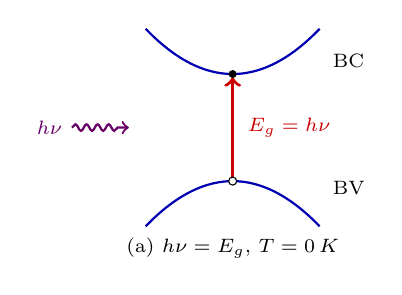
\begin{tikzpicture}[baseline=(current bounding box.center), scale=0.85, font=\footnotesize,
        photon/.style={->, thick, violet!80!black, decorate, decoration={snake, amplitude=1.2pt, segment length=4pt, post length=3pt}}]
        \draw[blue!70!black, thick, smooth, samples=30, domain=-1.3:1.3] plot (\x, {0.4*\x*\x + 1.6});
        \draw[blue!70!black, thick, smooth, samples=30, domain=-1.3:1.3] plot (\x, {-0.4*\x*\x});
        \node[anchor=west, font=\scriptsize] at (1.35, 1.8) {BC};
        \node[anchor=west, font=\scriptsize] at (1.35, -0.1) {BV};
        \draw[->, very thick, red!80!black] (0, 0) -- (0, 1.55);
        \node[anchor=west, font=\scriptsize, red!80!black] at (0.08, 0.8) {\( E_g = h\nu \)};
        \draw[photon] (-2.4, 0.8) -- (-1.55, 0.8);
        \node[anchor=east, font=\scriptsize, violet!80!black] at (-2.4, 0.8) {\( h\nu \)};
        \fill (0, 1.6) circle (1.7pt);
        \draw[fill=white] (0, 0) circle (1.7pt);
        \node[font=\scriptsize, anchor=north] at (0, -0.7) {(a) \( h\nu = E_g \), \( T = 0\,\text{K} \)};
    \end{tikzpicture}
    \hfill
    % --- Panel 2: hν > E_g, T > 0 K ---
    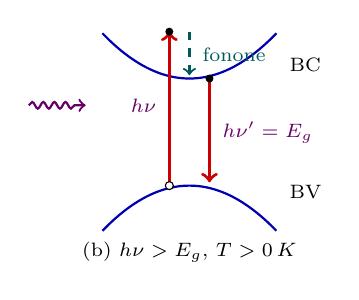
\begin{tikzpicture}[baseline=(current bounding box.center), scale=0.85, font=\footnotesize,
        photon/.style={->, thick, violet!80!black, decorate, decoration={snake, amplitude=1.2pt, segment length=4pt, post length=3pt}}]
        \draw[blue!70!black, thick, smooth, samples=30, domain=-1.3:1.3] plot (\x, {0.4*\x*\x + 1.6});
        \draw[blue!70!black, thick, smooth, samples=30, domain=-1.3:1.3] plot (\x, {-0.4*\x*\x});
        \node[anchor=west, font=\scriptsize] at (1.35, 1.8) {BC};
        \node[anchor=west, font=\scriptsize] at (1.35, -0.1) {BV};
        \draw[->, very thick, red!80!black] (-0.3, 0) -- (-0.3, 2.3);
        \node[anchor=east, font=\scriptsize, violet!80!black] at (-0.35, 1.2) {\( h\nu \)};
        \draw[->, thick, teal!70!black, dashed] (0.0, 2.3) -- (0.0, 1.65);
        \node[anchor=west, font=\scriptsize, teal!70!black] at (0.05, 1.95) {fonone};
        \draw[->, very thick, red!80!black] (0.3, 1.6) -- (0.3, 0.05);
        \node[anchor=west, font=\scriptsize, violet!80!black] at (0.35, 0.8) {\( h\nu' = E_g \)};
        \draw[photon] (-2.4, 1.2) -- (-1.55, 1.2);
        \fill (-0.3, 2.3) circle (1.7pt);
        \fill (0.3, 1.6) circle (1.7pt);
        \draw[fill=white] (-0.3, 0) circle (1.7pt);
        \node[font=\scriptsize, anchor=north] at (0, -0.7) {(b) \( h\nu > E_g \), \( T > 0\,\text{K} \)};
    \end{tikzpicture}
    \hfill
    % --- Panel 3: hν < E_g, T > 0 K ---
    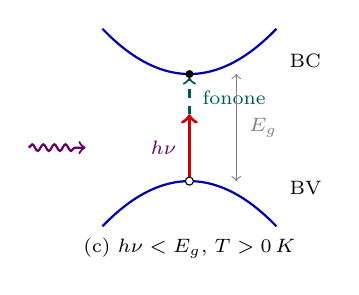
\begin{tikzpicture}[baseline=(current bounding box.center), scale=0.85, font=\footnotesize,
        photon/.style={->, thick, violet!80!black, decorate, decoration={snake, amplitude=1.2pt, segment length=4pt, post length=3pt}}]
        \draw[blue!70!black, thick, smooth, samples=30, domain=-1.3:1.3] plot (\x, {0.4*\x*\x + 1.6});
        \draw[blue!70!black, thick, smooth, samples=30, domain=-1.3:1.3] plot (\x, {-0.4*\x*\x});
        \node[anchor=west, font=\scriptsize] at (1.35, 1.8) {BC};
        \node[anchor=west, font=\scriptsize] at (1.35, -0.1) {BV};
        \draw[->, very thick, red!80!black] (0, 0) -- (0, 1.0);
        \node[anchor=east, font=\scriptsize, violet!80!black] at (-0.05, 0.5) {\( h\nu \)};
        \draw[->, thick, teal!70!black, dashed] (0, 1.0) -- (0, 1.55);
        \node[anchor=west, font=\scriptsize, teal!70!black] at (0.05, 1.25) {fonone};
        \draw[<->, thin, gray] (0.7, 0) -- (0.7, 1.6);
        \node[anchor=west, font=\scriptsize, gray] at (0.75, 0.8) {\( E_g \)};
        \draw[photon] (-2.4, 0.5) -- (-1.55, 0.5);
        \fill (0, 1.6) circle (1.7pt);
        \draw[fill=white] (0, 0) circle (1.7pt);
        \node[font=\scriptsize, anchor=north] at (0, -0.7) {(c) \( h\nu < E_g \), \( T > 0\,\text{K} \)};
    \end{tikzpicture}
    \caption{Tre scenari di interazione fotone-cristallo a seconda del rapporto fra \( h\nu \) ed \( E_g \).}
    \label{fig:assorbimento_emissione_fononi}
\end{figure}

\textbf{Caso (a): \( h\nu = E_g \) a \( T = 0\,\text{K} \).} Il fotone trasferisce esattamente l'energia del gap a un elettrone della banda di valenza, che salta direttamente in banda di conduzione senza coinvolgere fononi. L'elettrone eccitato può poi ricombinarsi tornando in BV ed emettendo un fotone della stessa energia \( h\nu = E_g \). È il caso ideale di pura assorbimento e riemissione ottica.

\textbf{Caso (b): \( h\nu > E_g \) a \( T > 0\,\text{K} \).} Il fotone porta più energia di quella strettamente necessaria per superare il gap: l'elettrone viene promosso ad uno stato sopra il fondo di BC, e l'eccesso \( h\nu - E_g \) viene smaltito sotto forma di un fonone (\textbf{emissione di fonone}). L'elettrone decade rapidamente al minimo di BC, e da lì può ricombinarsi con BV emettendo un fotone secondario di energia \( h\nu' = E_g \), inferiore a quella del fotone incidente. L'energia in eccesso si è dunque trasformata in vibrazione del reticolo.

\textbf{Caso (c): \( h\nu < E_g \) a \( T > 0\,\text{K} \).} Il fotone, da solo, non avrebbe energia sufficiente per superare il gap. A temperatura finita, però, il cristallo è popolato da fononi termicamente eccitati: l'assorbimento simultaneo di un fotone e di un fonone (\textbf{assorbimento di fonone}) fornisce all'elettrone l'energia mancante, e ne consente la transizione BV \( \to \) BC. Anche qui la luce riemessa nella successiva ricombinazione avrà in generale energia diversa da quella del fotone incidente.
\end{example}

\section{Energia interna, polarizzazioni e statistica dei fononi}

Le vibrazioni del reticolo non sono il prodotto di un'unica sorgente: possono essere indotte da onde di pressione (vibrazioni acustiche imposte dall'esterno), dall'agitazione termica del materiale a temperatura finita, o ancora dall'interazione con la radiazione elettromagnetica vista nel paragrafo precedente. In tutti questi casi, l'energia complessivamente immagazzinata nel reticolo si ottiene sommando i contributi di tutti i modi normali eccitati.

Tenendo conto del fatto che ogni atomo può vibrare lungo \emph{tre} direzioni spaziali indipendenti, esistono per ogni vettore d'onda \( \vec{k} \) tre distinti modi normali, uno per ciascun \textbf{stato di polarizzazione} \( p \); a ciascun modo è associata una sua pulsazione \( \omega_p(\vec{k}) \). L'energia interna vibrazionale del cristallo si scrive allora come somma su tutti i vettori d'onda e su tutte le polarizzazioni:

\begin{importantbox}
    \begin{equation}
        U_{\text{int}}(T) = \sum_{\vec{k}} \sum_{p} \hbar \omega_p(\vec{k}) \, N_p(\vec{k}),
    \end{equation}
\end{importantbox}

dove \( \hbar \omega_p(\vec{k}) \) è l'energia di un singolo fonone nel modo \( (\vec{k}, p) \), ed \( N_p(\vec{k}) \) è il numero di fononi presenti in quel modo. Si ricordi che il singolo modo è quantizzato secondo l'oscillatore armonico, \( E = \hbar \omega_0(n_{\vec{k}} + 1/2) \), dove \( n_{\vec{k}} \) è proprio il numero di occupazione (a meno dell'energia di punto zero).

\begin{note}{I fononi sono bosoni}{nota:fononi_bosoni}
I fononi sono particelle a spin intero (in particolare, hanno spin nullo): si comportano dunque come \textbf{bosoni}, e non c'è alcun limite al numero che può occupare uno stesso modo \( (\vec{k}, p) \). All'equilibrio termico a temperatura \( T \), il numero medio di fononi in un modo di pulsazione \( \omega \) è dato dalla \textbf{distribuzione di Bose-Einstein}:

\begin{equation}
    \bar{N}(\omega, T) = \frac{1}{e^{\hbar \omega / k_B T} - 1}.
\end{equation}

Questo risultato è ricavato in dettaglio nella meccanica statistica, e qui lo assumiamo come noto.
\end{note}

\section{Condizioni periodiche di Born-von Kármán}

Il modello di catena lineare considerato finora è formalmente infinito: ma nella realtà ogni cristallo ha dimensioni finite. Per gestire questo aspetto senza introdurre complicazioni dovute alla presenza di superfici, si adottano le \textbf{condizioni periodiche di Born-von Kármán}: si immagina di richiudere la catena su sé stessa, identificando l'atomo \( N+1 \) con l'atomo \( 1 \). In tre dimensioni, equivale a considerare il cristallo come un toro di lato pari alla sua dimensione fisica \( L \).

\begin{figure}[htbp]
    \centering
    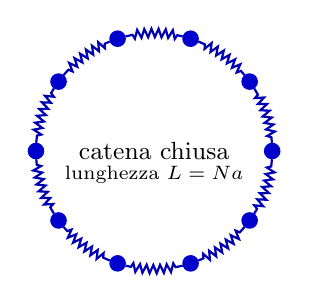
\begin{tikzpicture}[>=stealth, scale=1.0,
        spring/.style={decorate, decoration={zigzag, segment length=2.5pt, amplitude=1.5pt, pre length=2pt, post length=2pt}, thick}]
        \def\R{1.5}
        \foreach \i in {0, 1, ..., 9} {
            \pgfmathsetmacro{\ang}{\i*36}
            \pgfmathsetmacro{\angn}{(\i+1)*36}
            \draw[spring, blue!70!black] ({\R*cos(\ang+4)}, {\R*sin(\ang+4)}) arc[start angle={\ang+4}, end angle={\angn-4}, radius=\R];
        }
        \foreach \i in {0, 1, ..., 9} {
            \pgfmathsetmacro{\ang}{\i*36}
            \fill[blue!80!black] ({\R*cos(\ang)}, {\R*sin(\ang)}) circle (3pt);
        }
        \node[font=\small, anchor=center] at (0, 0) {catena chiusa};
        \node[font=\scriptsize, anchor=center] at (0, -0.3) {lunghezza \( L = N a \)};
    \end{tikzpicture}
    \caption{Catena di \( N \) atomi richiusa su sé stessa secondo le condizioni di Born-von Kármán.}
    \label{fig:born_von_karman}
\end{figure}

L'imposizione della periodicità rende la funzione d'onda invariante per una traslazione di \( L = N a \), e ciò significa che la sua fase deve essere riprodotta dopo aver percorso un'intera lunghezza della catena:

\begin{equation}
    e^{i k_x \cdot a} = e^{i k_x N a} = 1.
\end{equation}

Questa condizione \textbf{quantizza} i valori ammessi di \( k_x \), che possono assumere solo i valori discreti:

\begin{equation}
    k_x = \frac{2 \pi n}{L} = \frac{2 \pi n}{N a}, \qquad n \in \mathbb{Z}.
\end{equation}

Nella prima zona di Brillouin si contano dunque esattamente \( N \) valori distinti di \( k_x \): tanti quanti gli atomi (o, in generale, le celle) della catena.

\begin{note}{Dal discreto al continuo}{nota:somma_integrale}
Per un materiale \emph{macroscopicamente esteso}, \( N \) è enorme e i valori ammessi di \( k_x \) sono talmente fitti e vicini fra loro da poter essere trattati come una variabile continua. La somma sui modi si converte allora naturalmente in un integrale:

\begin{equation}
    \sum_{\vec{k}} \;\longrightarrow\; \frac{V}{(2\pi)^d} \int \dd^d k,
\end{equation}

dove \( V \) è il volume del cristallo e \( d \) la dimensionalità. Operativamente, per un materiale infinitamente esteso conviene contare gli \emph{stati che una particella può occupare} (cioè i valori ammessi di \( \vec{k} \)) piuttosto che le particelle stesse: è il punto di vista naturale della meccanica statistica nello spazio dei modi.
\end{note}

